\chapter{Validation et détails d'implémentation}

\section{Vue d'ensemble de la solution proposée}

Comme on le voit \ref{archi}

\begin{wrapfigure}{r}{.7\textwidth}
    \centering
    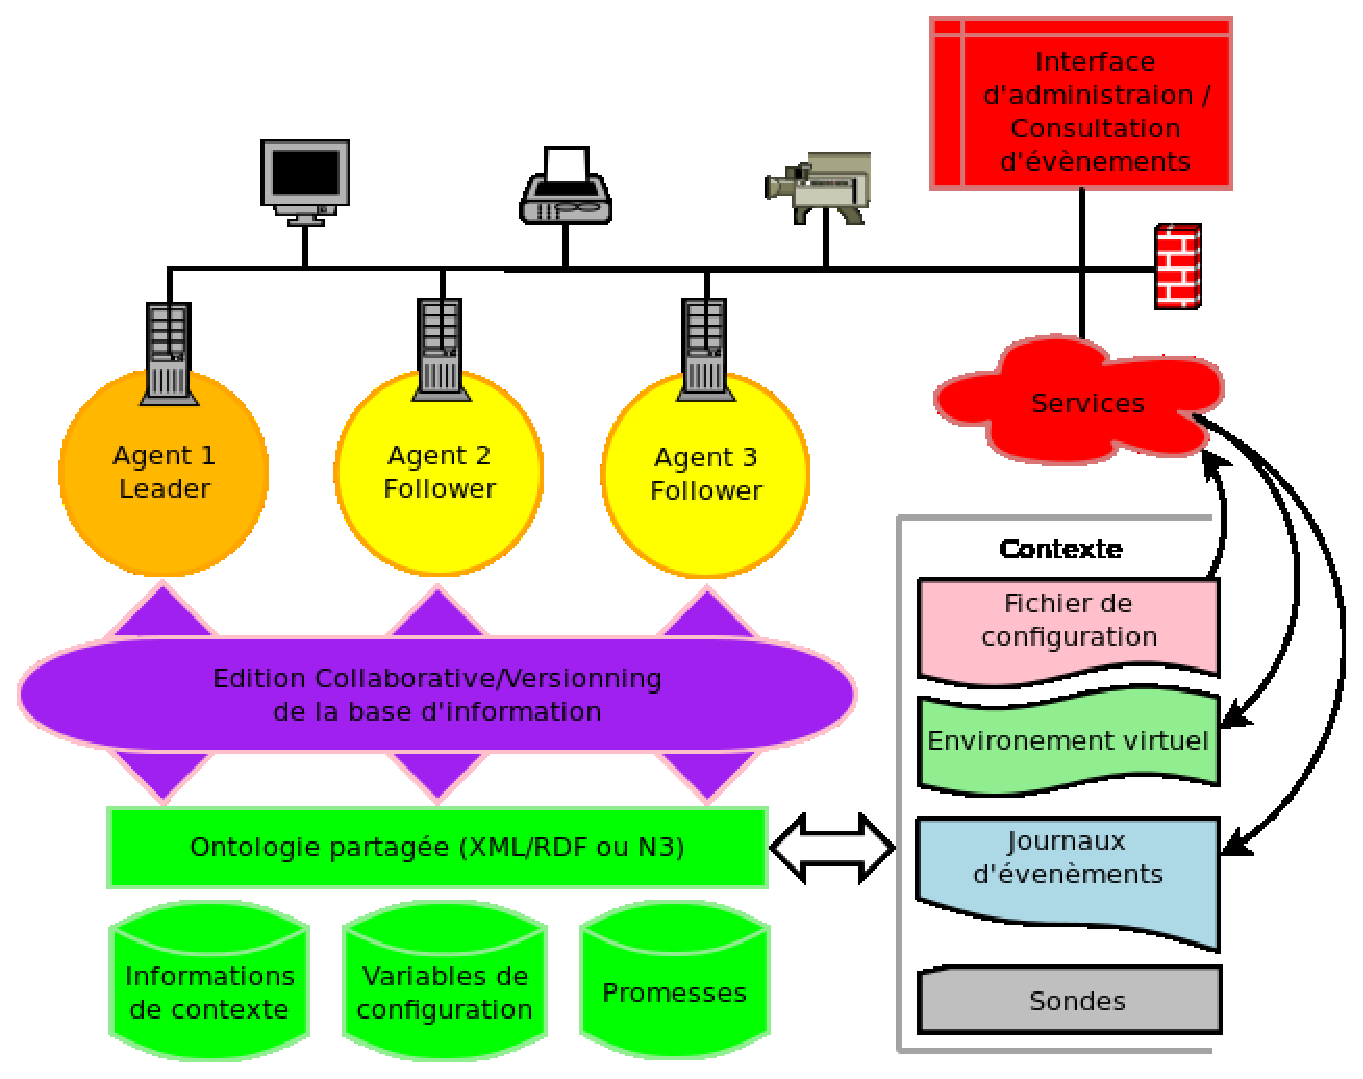
\includegraphics[width=.67\textwidth]{img/archi}
    \caption{Schéma d'implémentation du système multi-agents}
    \label{archi}
\end{wrapfigure}

%\begin{figure}[ht!]
%  \centering
%  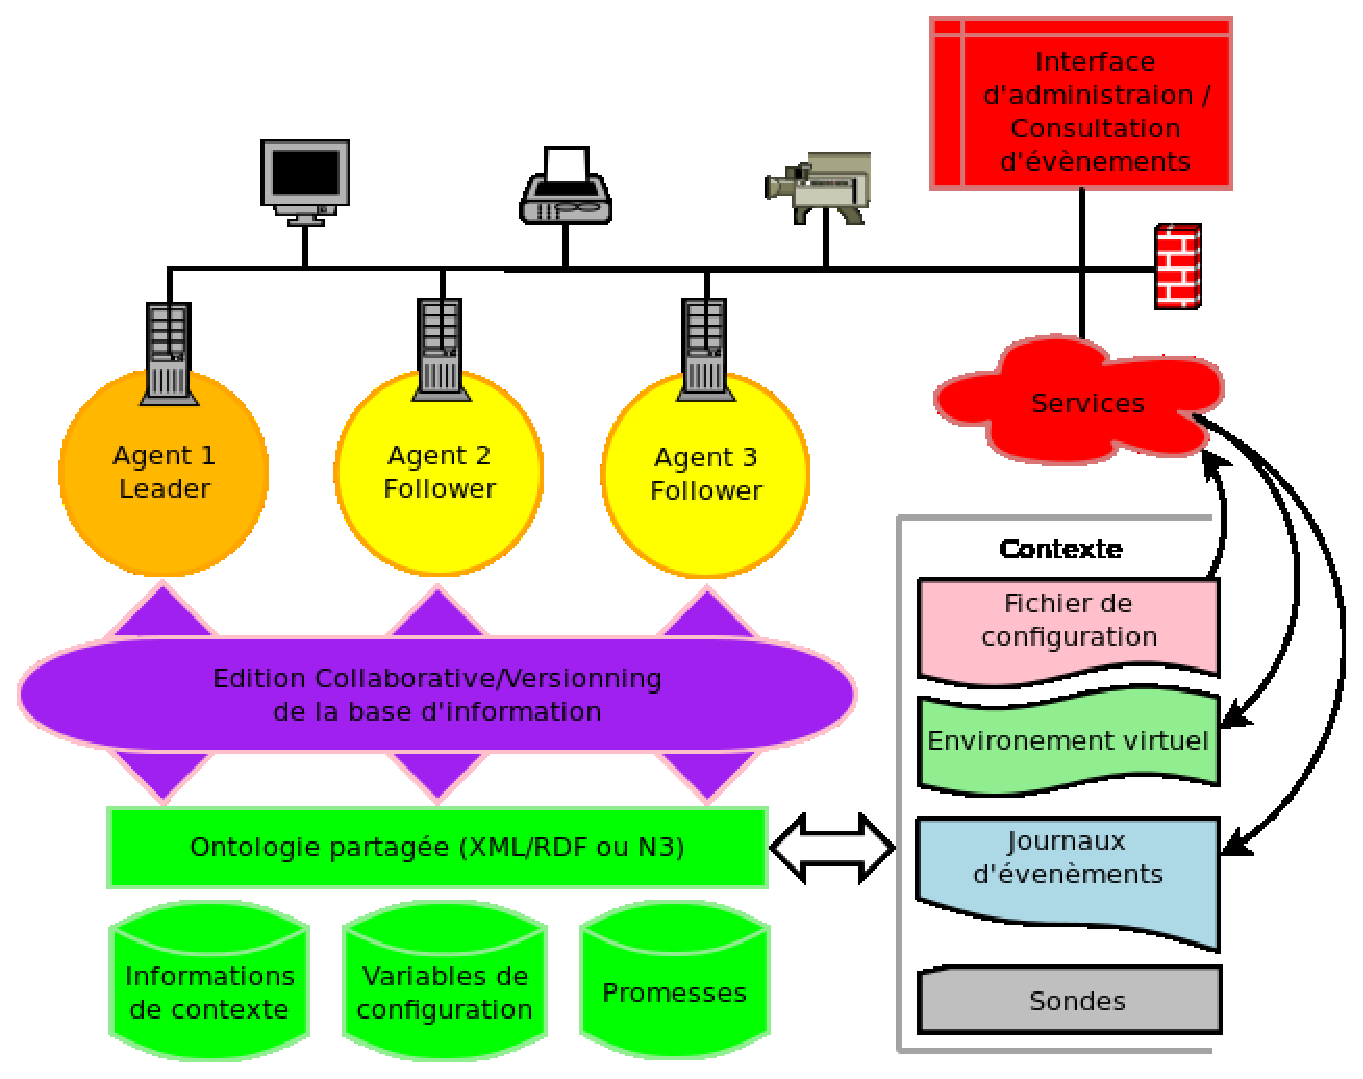
\includegraphics[width=120mm]{img/archi}
%  \caption{Schéma d'implémentation du système multi-agents}
%  \label{archi}
%\end{figure}

\section{Framework de gestion de configuration}

La gestion de la configuration est le processus de contraindre le comportement
d'un réseau de machines de manière à ce que le comportement de chaque machine
soit conforme aux politiques et lignes directrices prédéfinies, et
accomplisse les objectifs d'entreprise prédéterminés. Cela implique :

\begin{itemize}
  \item Des personnes
  \item Outil gestion de configuration ``zéro`` (exemple: CfEngine)
  \item Un ensemble ce machines interconnectées
  \item Un ensemble de processus de configuration destiné à aboutir à un système
	  conforme à la politique en vigueur.
\end{itemize}

Les paramètres de configuration peuvent être la permission d'un fichier,
l'adresse d'un carte réseau, le type de système de fichier pouvant être monté
sur un volume disque.

La possibilité d'automatiser la configuration des réseaux IP (Internet
Protocol) en utilisant une technologie sémantique est également très
prometteuse. L'initiative connexe de créer un environnement de réseau de
capteurs basé sur le ontologies semble également être une solution viable.

La plupart des organisations aujourd'hui n'ont aucun procédé systématique pour
gérer leurs informations de configuration. Cela signifie que des informations
comme l'adresse IP d'une machine et le statut de son service réseau sont
stockées de manière dispersée et désorganisée. Certains outils de supervision
tels que Nagios présente une manière de réorganiser ces informations provenant
de sources dispersées.

L'idée d'utiliser une CMDB (Configuration Management Database) est également un
alternative permettant de solutionner le problème ci-dessus. Toutefois, le besoin
pour un gestionnaire d'informations de plus haut niveau est mentionné dans de
nombreuses littératures.

Cette nouvelle façon de renforcer l'efficacité de la gestion des connaissances
dans le domaine de la gestion de configuration, nécessite la possibilité
d'extraction automatique de données à partir d'emplacements de stockage
précédents et la possibilité de mise à jour automatique de stockages permanents
tels que la CMDB afin d'augmenter la qualité de l'information sous-jacente.

La possibilité de ces deux fonctions à savoir, l'extraction automatique des
données et également la mise à jour automatique des informations stockées ont
été fournies par ITIL. % FIXME ITIL ?

Le travail de ce mémoire est de démontrer les possibilités d'obtenir un
gestionnaire de connaissances intégré en conjuguant les ontologies, la théorie
de la promesse et le consensus de Raft. La structure de l'information de
configuration stockée dans une CMDB et dans d'autres fichiers sera représentée en
concordance avec les standard de OWL. Cette structure de domaine de connaissance
sera implémentée comme une promesse de structure d'information.

\noindent\rule{8cm}{0.4pt}

La Configuration Management Database (abrégé CMDB), ou base de données de
gestion de configuration, est une base de données unifiant les composants d'un
système informatique. Elle permet de comprendre l'organisation entre ceux-ci et
de modifier leur configuration. La CMDB est un composant fondamental d'une
architecture ITIL.

\section{Ontologie pour un gestionnaire de configuration basé sur la théorie de
la promesse}


\begin{figure}
  \begin{verbatim}
  #include <iostream>
  int main(int argc, char** argv) {
    std::cout << "Hello World." << std::endl;
    return 0;
  }
  \end{verbatim}
  \caption{Example source code.}
  \label{fig:sourcecode}
\end{figure}

\section{Conclusion}

Les technologies basées sur le contexte vont jouer un rôle fondamental dans la
prochaine génération de systèmes informatiques à mesure que la complexité des
logiciels, la diversité et l'omniprésence des périphériques continuent
d'augmenter. Cependant, elle doivent offrir des mécanismes permettant la
gestion automatique des dépendances inter-composants et composant/ressource.
Dans le cas contraire, le développement de systèmes basés sur les composants
demeura difficile à appréhender et conduira bien souvent à des systèmes peu
fiables et pas assez robustes.

Les environnements qui composeront l'informatique ubiquitaire de demain sera
composé de milliers de périphériques, avec des millions de composantes
logicielles. Les systèmes actuels s'appuient fortement sur la configuration
manuelle, ce qui à un telle échelle n'est plus possible. Il n'existe que deux
issues possible à cette situation : une configuration statique, ou une
configuration dynamique et automatique. Puisque les environnements ont
tendance à être de plus en plus dynamiques, la configuration autonome semble
incarner la seule solution viable.

% ex: set spelllang=fr spell: %
%%% Local Variables: ***
%%% mode: latex ***
%%% TeX-master: "thesis.tex" ***
%%% End: ***
